% !TeX root = ./main.tex

\chapter{Navier-Stokes/Darcy 耦合模型的反问题实验}
传统的数值求解方法如有限元、格子波尔兹曼方法等,当流体力学物理模型的方程发生改变时,这些方法往往要进行较大幅度的改动或重新设计,而本文提出的神经网络求解算法只需要对损失函数做出细微的调整便可以在不同方程中进行迁移。

另一方面,流体力学领域还存在各种各样的反问题,比如物理模型的初边值条件是未知的,取而代之的是已知内部部分区域或部分物理量的数值真解,以此反推整个区域的流体运动情况;或者,物理模型的方程本身具有一些未知参数,需要通过真实的数值结果进行反推。这类问题在工程应用中具有很大意义,然而各种传统方法对此类问题的求解具有一定的难度,在本文神经网络求解的框架下,却很容易对该类反问题尝试进行求解。

因此,本章设计了三个数值实验,分别为区域反问题实验、物理量反问题实验以及方程参数反问题实验,通过这些实验验证 cPINNs 对各种类型反问题的求解潜力。


\section{区域反问题实验}

本节将计算一个区域反问题的算例,即求解时不提供初边值条件,而是选择空间区域中的一部分真解作为已知条件。该问题对应的神经网络求解算法的修改为将初边值区域的损失函数替换为自定义选择区域的物理量损失即可。算例将采取实验一 ~\eqref{eq:example1} 的解析解,而自定义区域设置为 $\Omega_{id}= \{ (x,y) \mid x \in [0.15,0.25] \cup [0.45,0.55] \cup [0.75,0.85]; y \in [0.15,0.25] \cup [0.45,0.55] \cup [0.75,0.85] \cup [1.15,1.25] \cup [1.45,1.55] \cup [1.75,1.85]) \}$,这是一种类似网格的子区域,如图 \ref{fig:example_area_inverse} 中实心部分所示:

\begin{figure}[H]
    \centering
    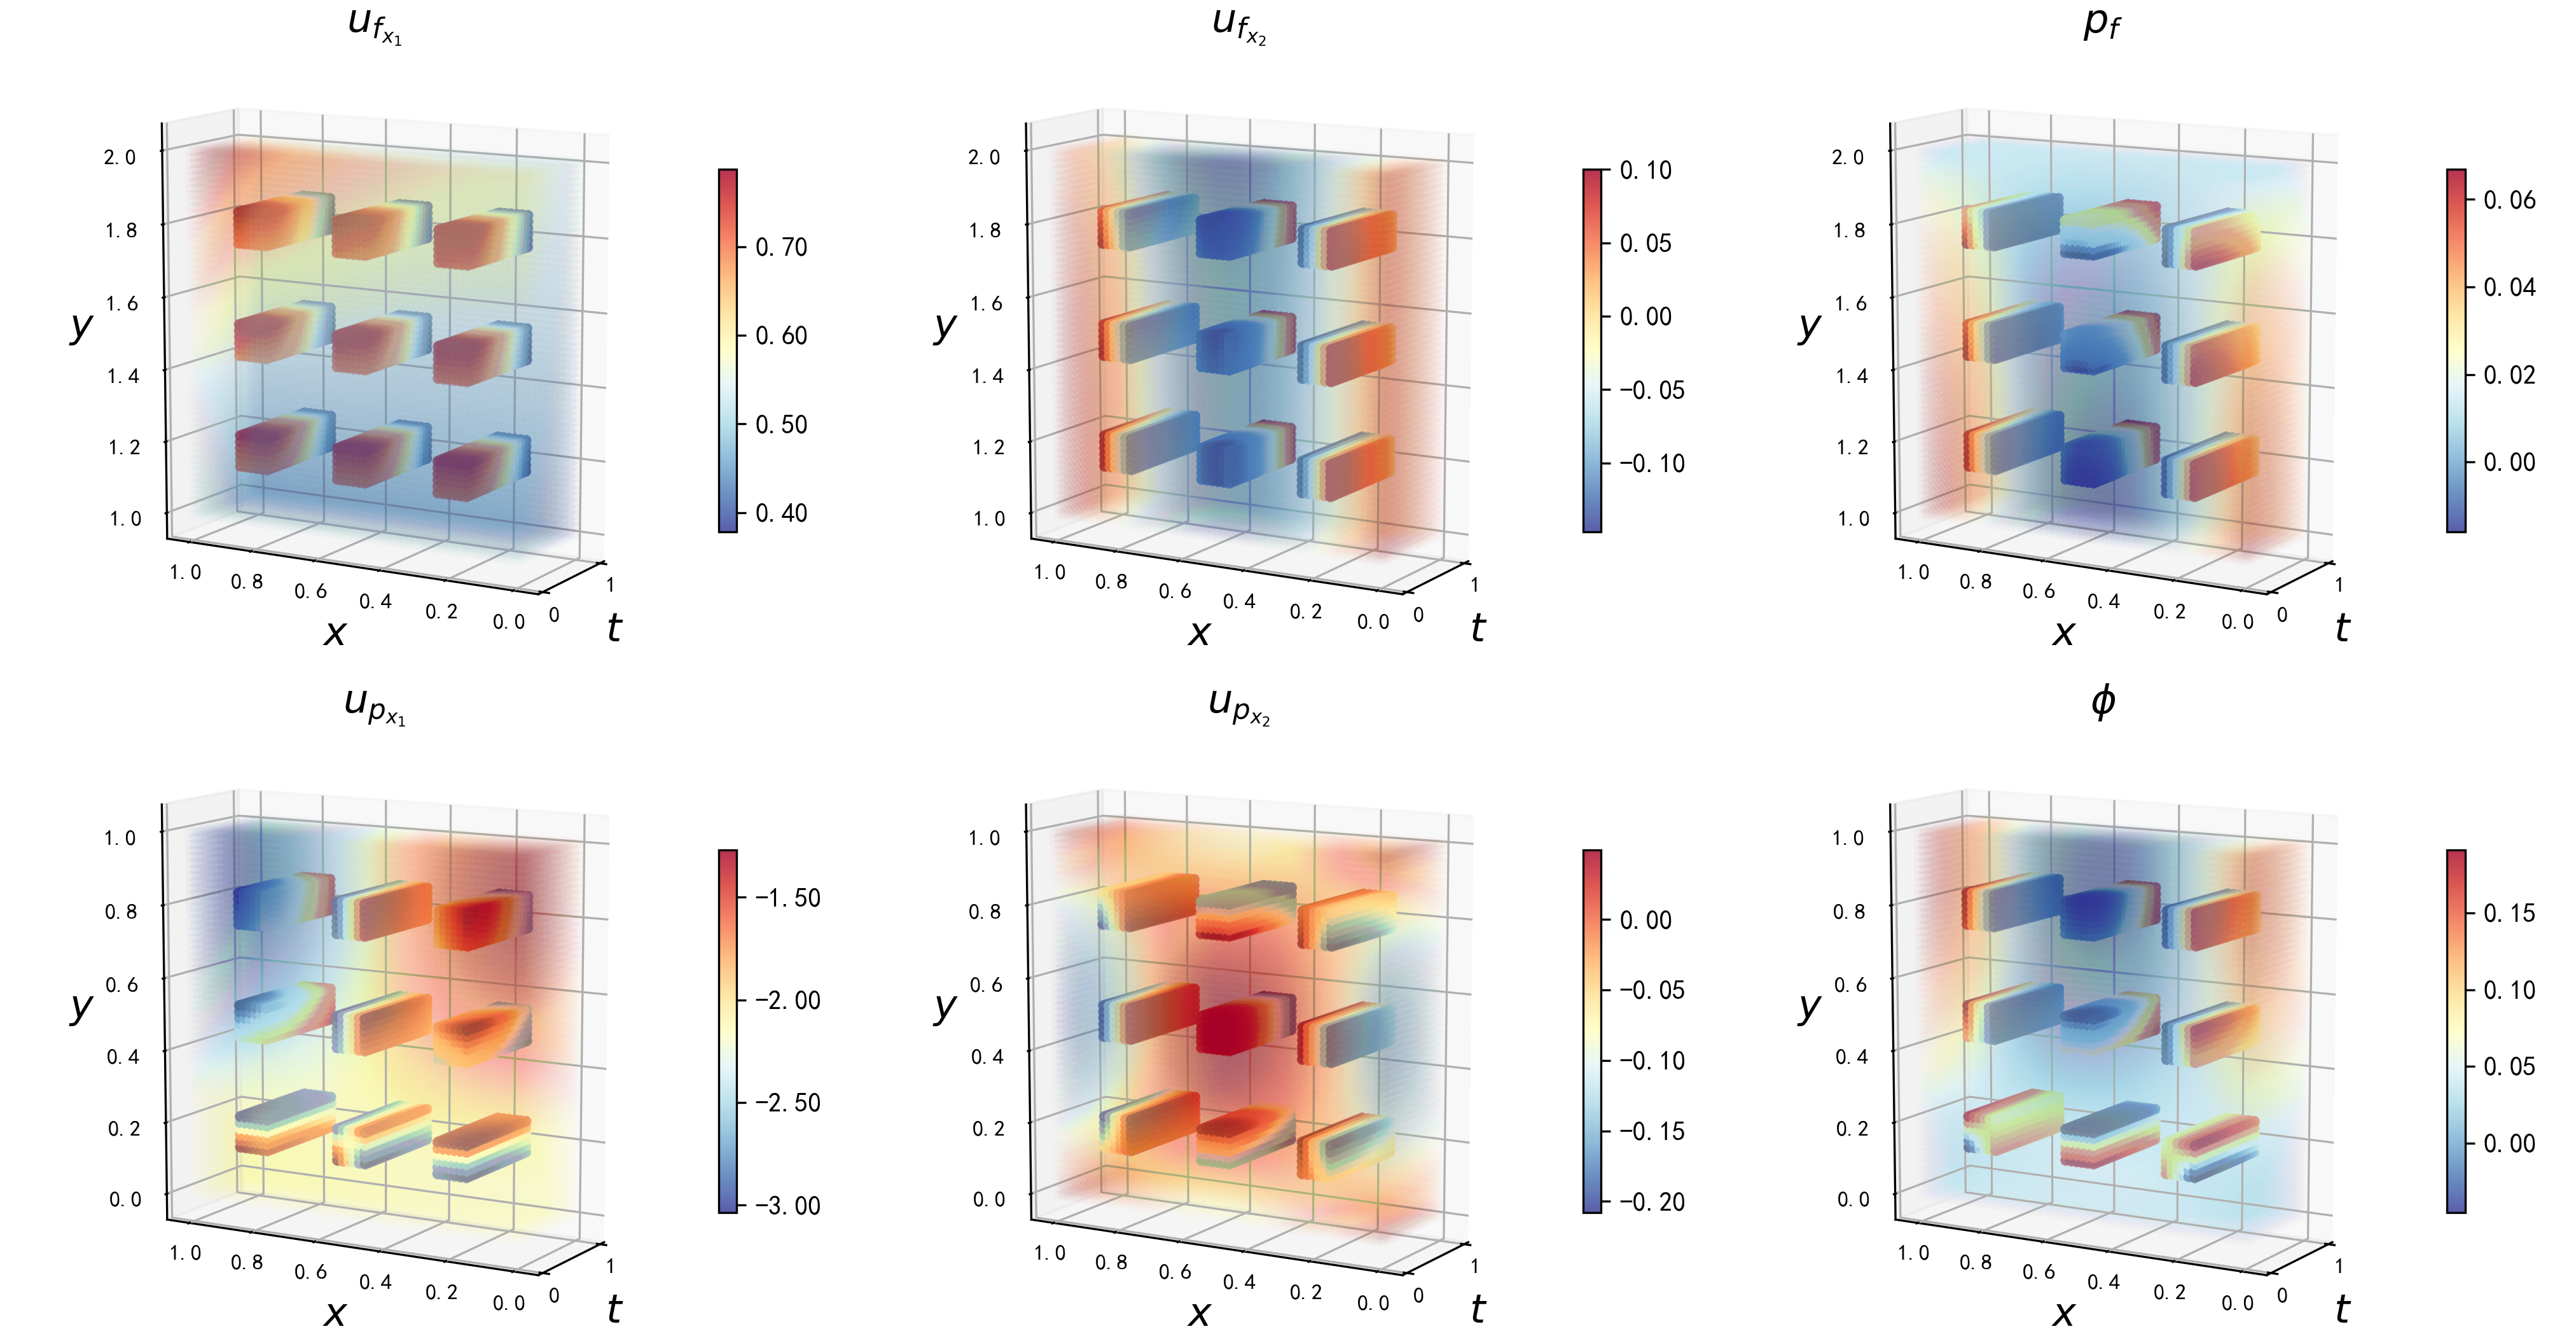
\includegraphics[width=0.75\linewidth]{images/example_area_inverse.png}
    % \caption*{}
    \caption{ 反问题的区域设置 }
    \label{fig:example_area_inverse}
\end{figure}

而相应地两区域对应的损失函数删掉了模型的初边值条件,添加上 $\Omega_{id}$ 对应的真值条件损失。网络结构等训练配置同上节保持不变,实验结果如表 \ref{tab:example_area_inverse} 所示:

\begin{table}[H]
    \centering
    \caption{区域反问题实验结果}
    \begin{tabular}{cccc}
        \toprule
        真解公式 & $\relaErr_{u}$ & $\relaErr_{p}$ \\
        \midrule
        公式 ~\eqref{eq:example1}  & $\num{2.7232}{-2}$ & $\num{6.0616}{-2}$ \\
        \bottomrule
    \end{tabular}
    \label{tab:example_area_inverse}
\end{table}

拟合结果如图 \ref{fig:example_area_inverse_fitted} 所示:

\begin{figure}[H]
    \centering
    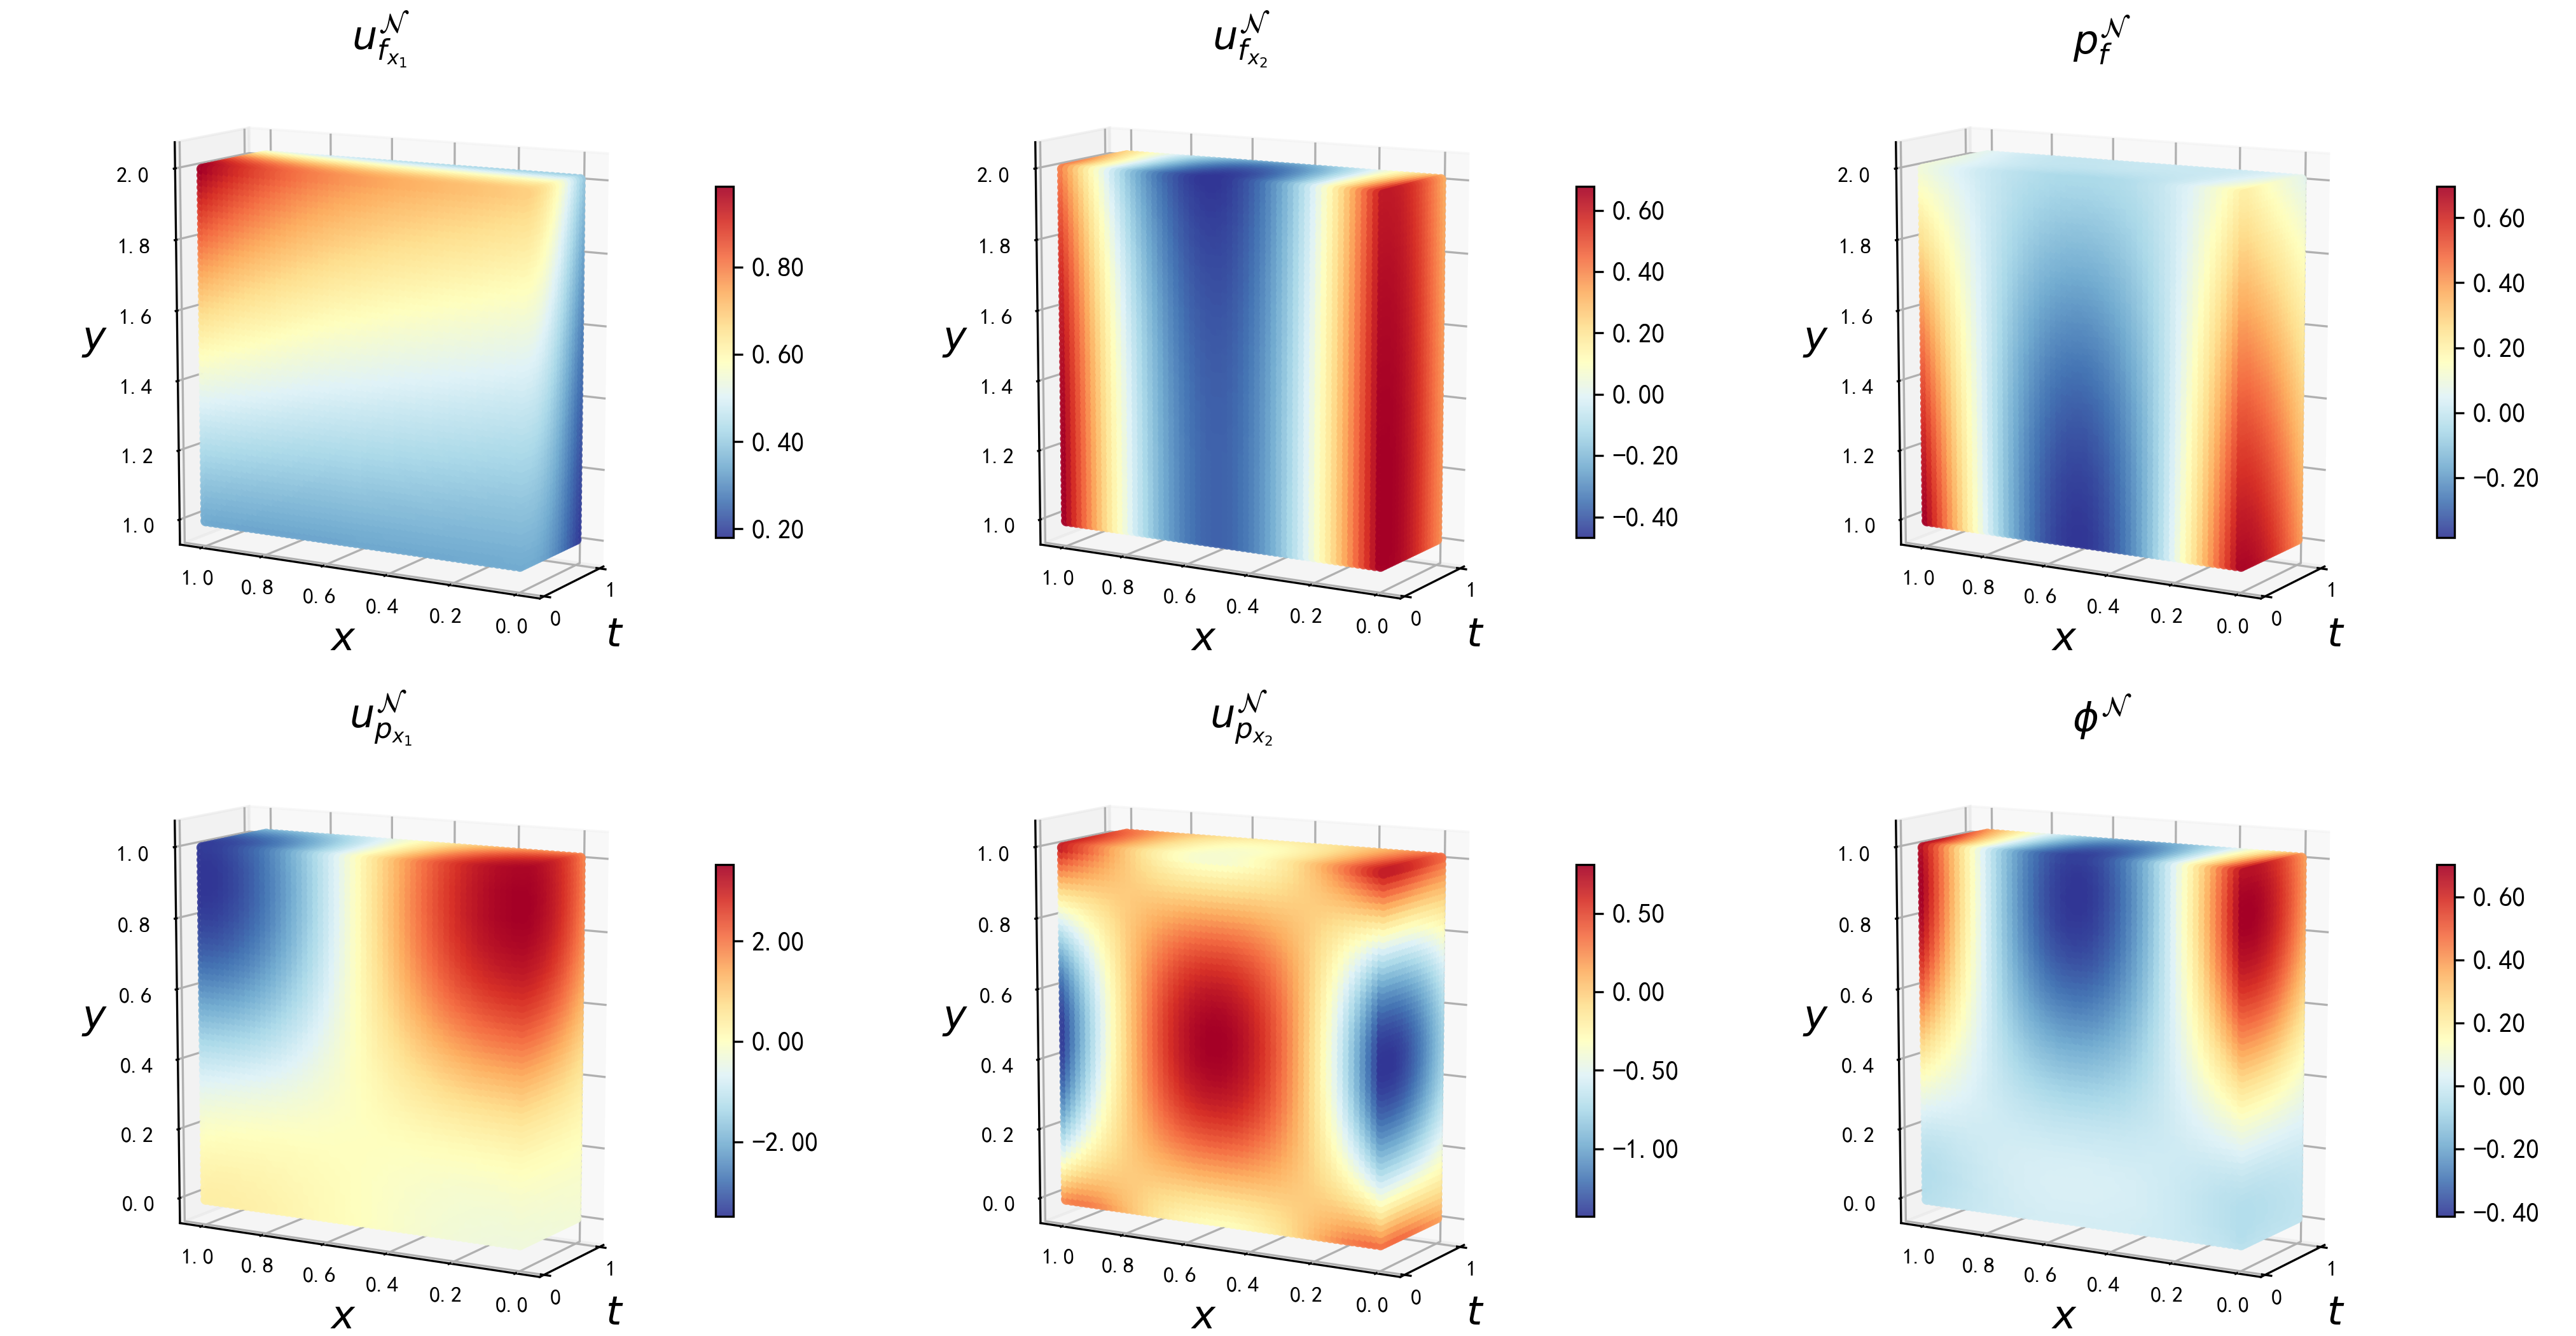
\includegraphics[width=0.75\linewidth]{images/example_area_inverse_fitted.png}
    % \caption*{}
    \caption{ 区域反问题实验结果图示 }
    \label{fig:example_area_inverse_fitted}
\end{figure}

可以看出对于上述区域设置,网络还是能够较好的还原出各物理量真解的。值得一提的是,在实验中发现并非任意的自定义区域均能使算法成功求解反问题,比如当区域选择过小,或者位置过于特殊时,算法虽然能够收敛,但网络拟合出的解析解将与真解差距过大,这提示该类反问题并非总是适定的(解的存在可能不唯一)。

\section{物理量反问题实验}

本节针对物理量反问题进行数值实验。所谓物理量反问题就是在不提供初边值条件的前提下,只提供部分物理量的全部信息来推断其他物理量的数值解。如隐藏型流体力学算法(Hidden fluid mechanics,HFM)\cite{raissi2020hidden} 就是只提供输运方程中标定物的物理量信息来反推出流场中的速度与压力场。由于本文耦合模型不涉及到输运问题,此物理量反问题实验将利用实验一 ~\eqref{eq:example1} 的真解,在求解上只提供两区域中代表压力的 $\pf^*, \pp^*$ 作为已知条件,目标是反推出模型中的速度场数值解。

类似区域反问题实验,cPINNs 迁移到此问题同样需要去除损失函数中的初边值部分,另外加入两区域压力物理量的损失部分。训练配置与上一个实验保持相同。实验结果见表 \ref{tab:example_phy_inverse}:

\begin{table}[H]
    \centering
    \caption{物理量反问题实验结果}
    \begin{tabular}{cccc}
        \toprule
        真解公式 & $\relaErr_{u}$ & $\relaErr_{p}$ \\
        \midrule
        公式 ~\eqref{eq:example1}  & $\num{8.5319}{-2}$ & $\num{2.1002}{-1}$ \\
        \bottomrule
    \end{tabular}
    \label{tab:example_phy_inverse}
\end{table}

同样地,拟合出的数值结果可视化展示如图 \ref{fig:example_phy_inverse_fitted}:

\begin{figure}[H]
    \centering
    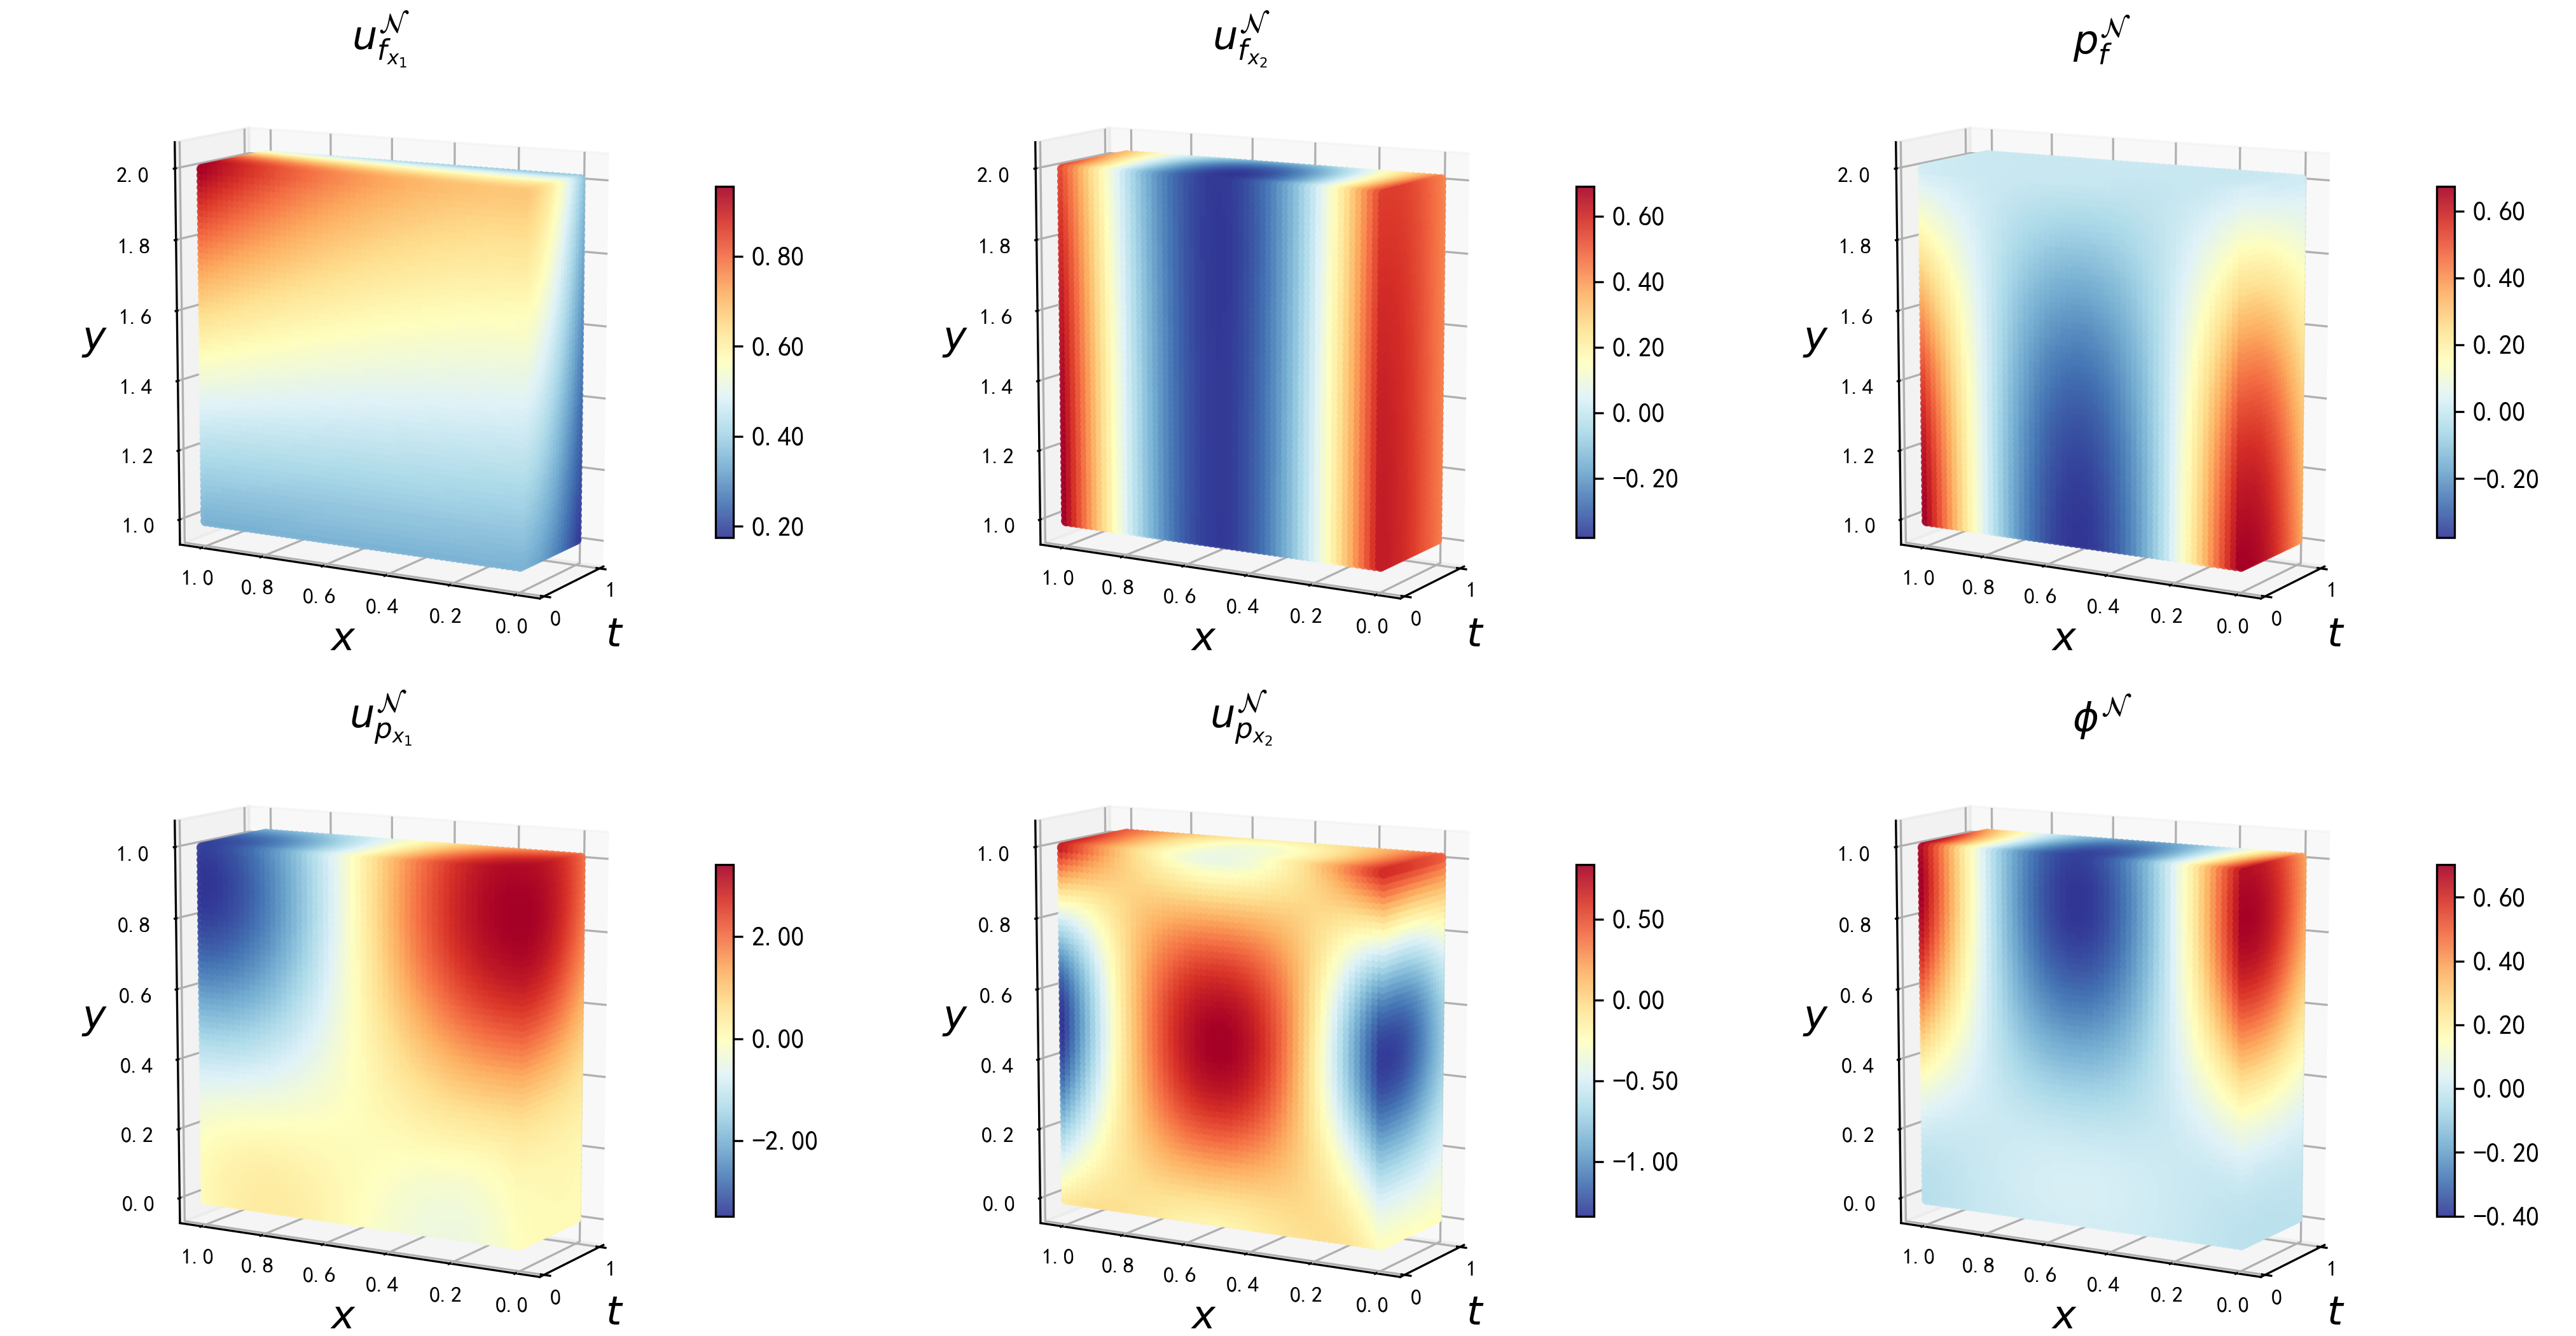
\includegraphics[width=0.75\linewidth]{images/example_phy_inverse_fitted.png}
    % \caption*{}
    \caption{ 物理量反问题的拟合效果 }
    \label{fig:example_phy_inverse_fitted}
\end{figure}

\section{方程参数反问题实验}

Navier-Stokes/Darcy 耦合模型物理公式中有一些参数如 $ \kappa, \alpha $ 需要通过实验确定,这就引出了关于未知方程参数的反问题,即已知全部或部分真解信息,反推出物理方程中的未知参数问题。本文的神经网络算法框架也能够尝试解决此类问题,具体做法为,将物理方程中的未知参数作为网络训练参数的一部分参与优化算法中进行更新即可,实践中现有的深度学习编程框架\footnote{本文算法的实现主要基于pytorch编程库}也不难做到这一点。

本节利用实验二的真解算例来测试神经网络算法解决方程参数反问题的能力。实验令已知条件为全部数值真解,而把耦合模型方程中的参数 $ \kappa, \alpha $ 设为未知量,加入到网络待训练参数中去。此时算法 \ref{algo:main} cPINNs 中的损失函数变为公式 ~\eqref{eq:example_param_inverse},注意这里还将 $\Lossf$ 与 $\Lossp$ 中的初边值条件损失修改为全部数值真解条件的损失(对应训练集为 $\TDf^*$,$\TDp^*$,$\TiBD^*$ )。最后迁移后的 cPINNs 算法流程见图 \ref{fig:param_inverse_cPINNs}。

\begin{equation}\label{eq:example_param_inverse}
    \begin{aligned}
        &\Loss{total}{\params_f,\params_p,\kappa,\alpha}{\TDf^*,\TDp^*,\TiBD^*} \\
        =& \Loss{f}{\params_f}{\TDf^*} + \Loss{p}{\params_p, \kappa}{\TDp^*} + \Loss{\iB}{\params_f,\params_p, \alpha}{\TiBD^*}
    \end{aligned}
\end{equation}

\begin{figure}[H]
    \centering
    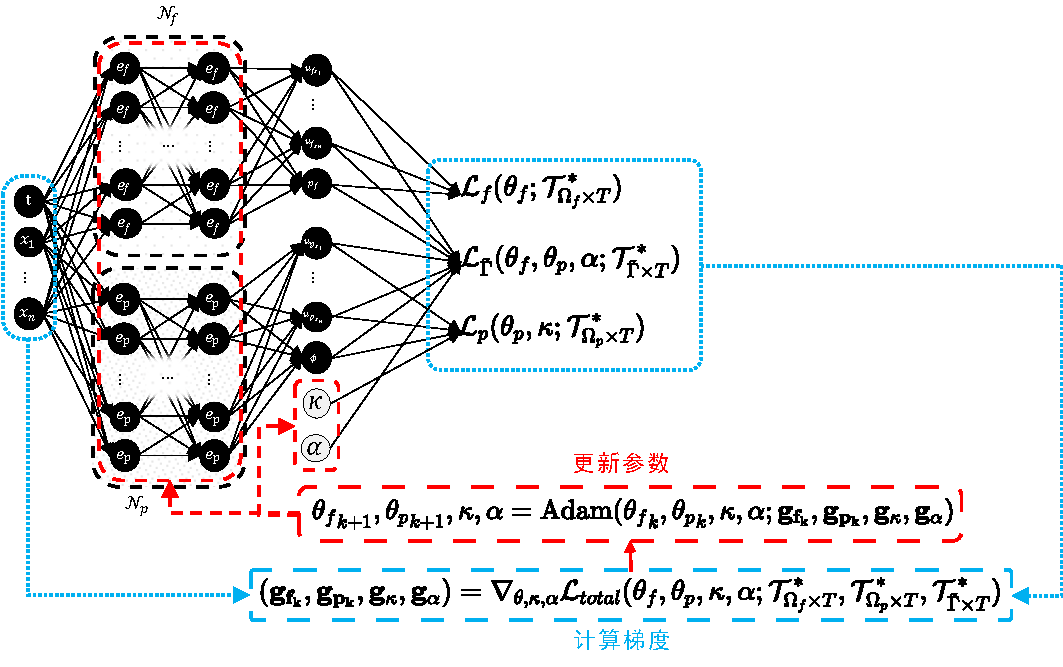
\includegraphics[width=1.0\linewidth]{images/参数反问题算法迁移图示.pdf}
    % \caption*{}
    \caption{ cPINNs 算法流程图示 }
    \label{fig:param_inverse_cPINNs}
\end{figure}

物理方程的其他参数设置以及训练的网络结构等参数配置与上节相同。拟合结果见表 \ref{tab:example_param_inverse},可以看出算法对各个参数的拟合效果都很好。

\begin{table}[H]
    \centering
    \caption{方程参数反问题实验结果}
    \begin{tabular}{ccccc}
        \toprule
        \multicolumn{2}{c}{真解} & \multicolumn{2}{c}{拟合值}\\ 
        \cmidrule(r){1-2} \cmidrule(r){3-4}
        $\kappa$ & $\alpha$ & $\kappa$ & $\alpha$ \\
        \midrule
        1.0   & 1.0 & $\num{0.99989}{0} $  & $\num{1.00001}{0}$ \\
        $\num{1}{-1}$ & 1.0 & $\num{0.99993}{-1}$  & $\num{1.00003}{0}$ \\
        $\num{1}{-2}$ & 1.0 & $\num{0.10032}{-2}$  & $\num{1.00011}{0}$ \\
        $\num{1}{-3}$ & 1.0 & $\num{0.10102}{-3}$  & $\num{1.00105}{0}$ \\
        $\num{1}{-6}$ & 1.0 & $\num{0.10379}{-6}$  & $\num{1.03007}{0}$ \\
        \bottomrule
    \end{tabular}
    \label{tab:example_param_inverse}
\end{table}



